\documentclass[handout]{beamer}
%\documentclass{beamer}
\usepackage{tikz}
\usetikzlibrary{positioning}
\usepackage[normalem]{ulem}
\usepackage{xcolor}
\usepackage{array}
\usepackage[backend=biber,citestyle=authoryear]{biblatex}
\addbibresource{ref.bib}

\usepackage{makecell}

\renewcommand\theadalign{bc}
\renewcommand\theadfont{\bfseries}
\renewcommand\theadgape{\Gape[4pt]}
\renewcommand\cellgape{\Gape[4pt]}


\tikzstyle{every picture}+=[remember picture]
\usetikzlibrary{positioning}
\usetikzlibrary{decorations.pathreplacing}

\usetheme{CambridgeUS}
\graphicspath{{figures/}}
\newcommand{\bvar}[1]{\mathbf{#1}} 
\definecolor{red}{HTML}{cf161e}
\definecolor{lgrey}{HTML}{dddddd}
\definecolor{bgray}{HTML}{E8E6E2}
\makeatletter
\setbeamertemplate{footline}
{
  \leavevmode%
  \hbox{%
  \begin{beamercolorbox}[wd=.5\paperwidth,ht=2.25ex,dp=1ex,center]{author in head/foot}%
    \usebeamerfont{author in head/foot}\insertshortauthor~~\beamer@ifempty{\insertshortinstitute}{}{(\insertshortinstitute)}
  \end{beamercolorbox}%
  \begin{beamercolorbox}[wd=.5\paperwidth,ht=2.25ex,dp=1ex,center]{date in head/foot}%
    \usebeamerfont{date in head/foot}\insertshorttitle{}
  \end{beamercolorbox}}%
  \vskip0pt%
}
\makeatother
   
\setbeamercolor{normal text}{fg=black,bg=white}
\setbeamercolor{block title}{bg=red,fg=white}
\setbeamercolor{block body}{bg=lgrey}
\setbeamercolor*{item}{fg=red}
\setbeamercolor{structure}{fg=red}
\setbeamercolor{background canvas}{parent=normal text}
\setbeamercolor{background}{parent=background canvas}
\setbeamercolor{frametitle}{fg=red}
\setbeamercolor{section in head/foot}{bg=red}
\setbeamercolor{author in head/foot}{bg=red}
\setbeamercolor{date in head/foot}{fg=red}


\title{\textcolor{red}{Bias-Variance Tradeoffs in Joint Spectral Embeddings}}
\author[Benjamin Draves]{Benjamin Draves \and Daniel Sussman}
\institute[Boston Univeristy] 
{\normalsize Boston University}

\date{Joint Statistical Meetings, 3 August 2020}

\begin{document}

\begin{frame}
  \titlepage
\end{frame}

%--------------------------------------------------------------
\section{Joint Network Embeddings}

\begin{frame}{Multiplex Networks}
\begin{itemize}
    \item Multiplex networks encode multiple relationships between entities as a collection of networks. 
    \begin{center}
        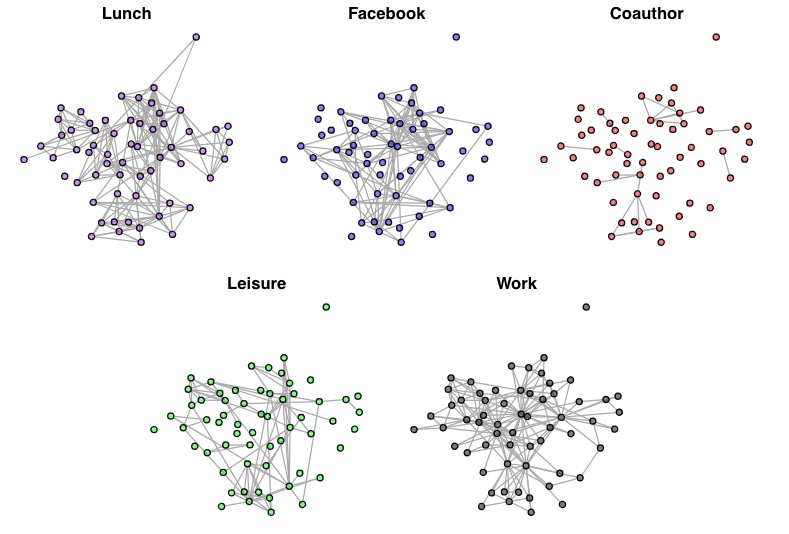
\includegraphics[width=0.6\textwidth]{aarhus_multiplex.jpg}
    \end{center}\pause
    \item Application areas; International Trade, Transportation Systems, Terrorist Groups, Neuroscience \parencite{Kivela2014}. 
\end{itemize}
\end{frame}

\begin{frame}{Individual Spectral Embeddings}
\begin{center}
    \begin{tikzpicture}
    %Draw Networks
    \node[shape=rectangle, align = center] (G1) at (-4,2.5) {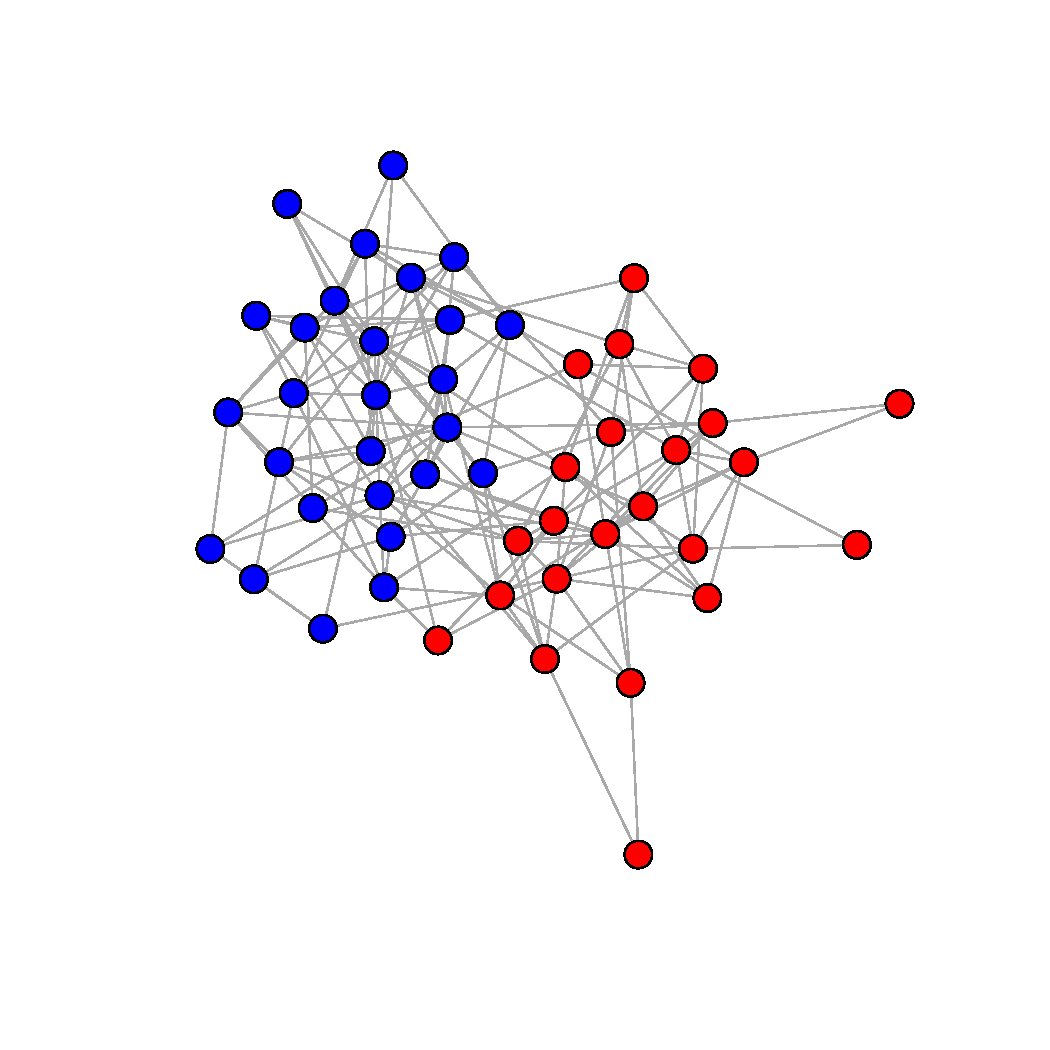
\includegraphics[width = 1in, height = 1in]{g1_beamer.pdf}};
    \node[shape=rectangle, align = center] (Gg) at (-4,0) {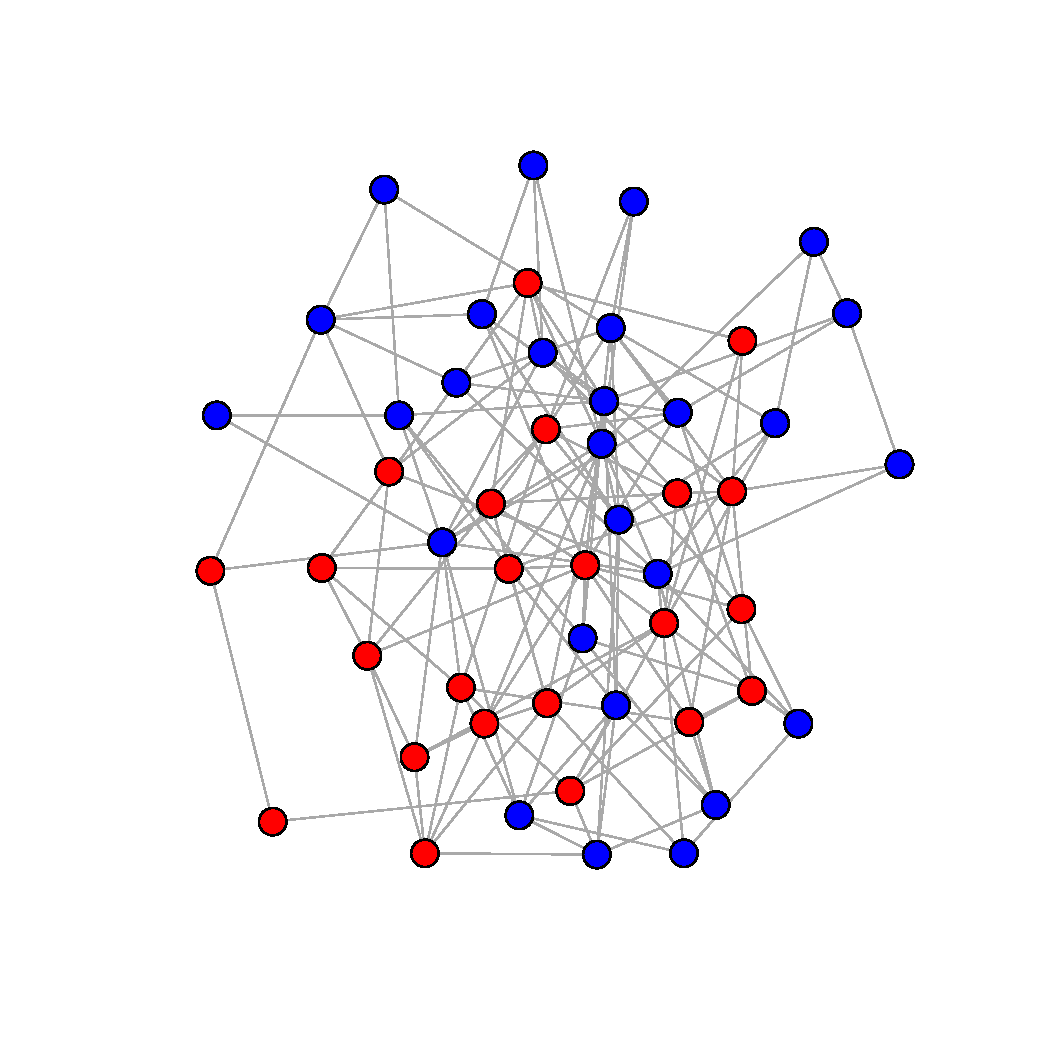
\includegraphics[width = 1in, height = 1in]{g2_beamer.pdf}};
    \node[shape=rectangle, align = center] (Gm) at (-4,-2.5) {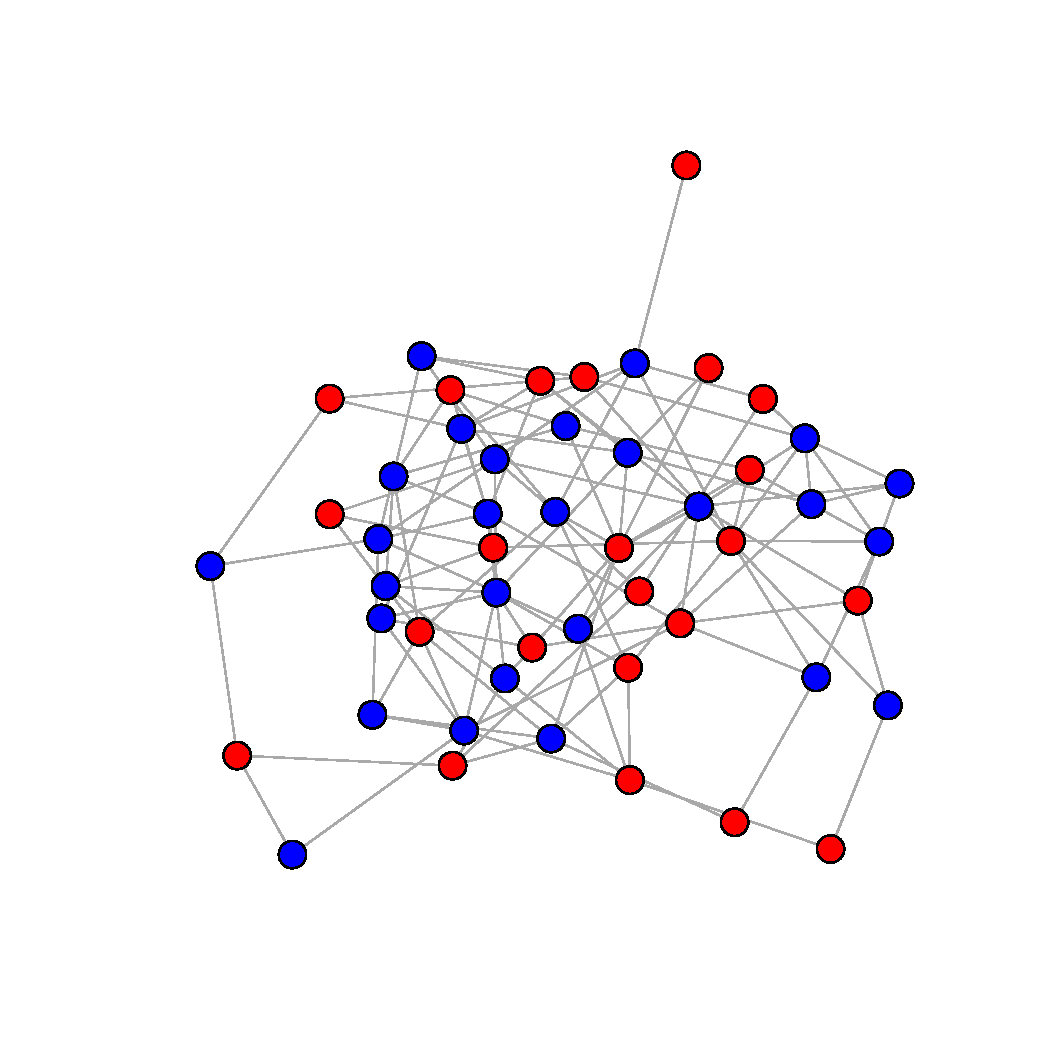
\includegraphics[width = 1in, height = 1in]{g3_beamer.pdf}};
    
    %Draw Adjacency Matrices
    \node[shape=rectangle, align = center] (A1) at (-2,2.5) {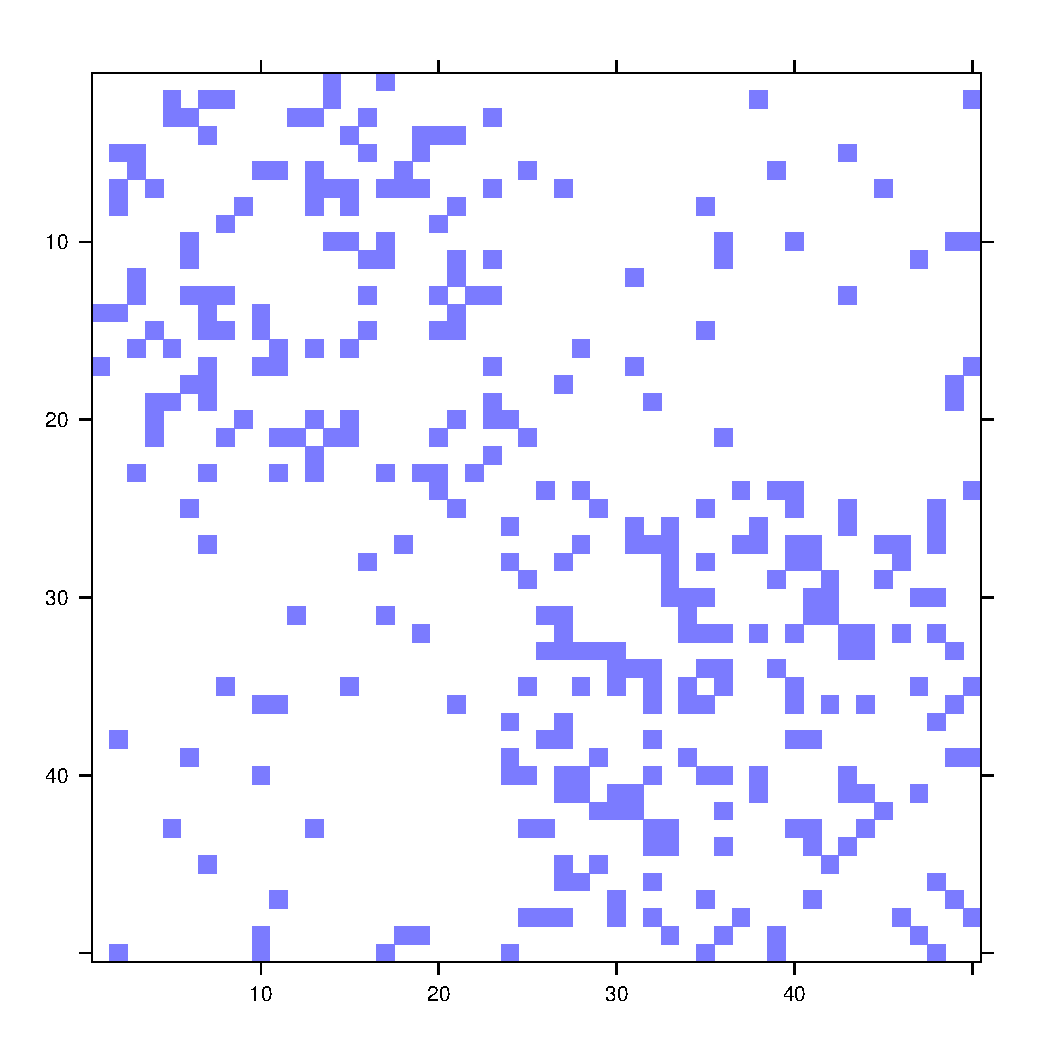
\includegraphics[width = .7in, height = .7in]{A1_beamer.pdf}};
    \node[shape=rectangle, align = center] (Ag) at (-2,0) {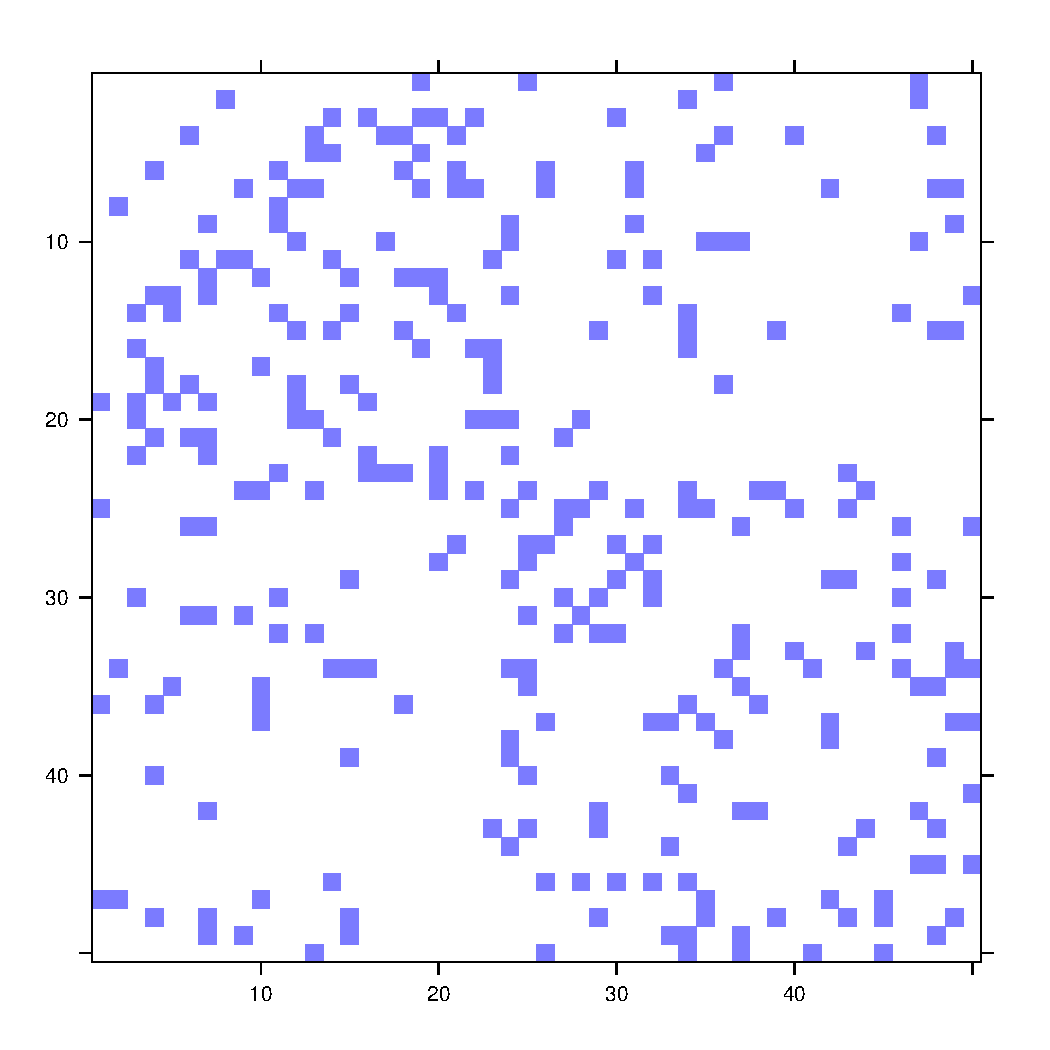
\includegraphics[width = .7in, height = .7in]{A2_beamer.pdf}};
    \node[shape=rectangle, align = center] (Am) at (-2,-2.5) {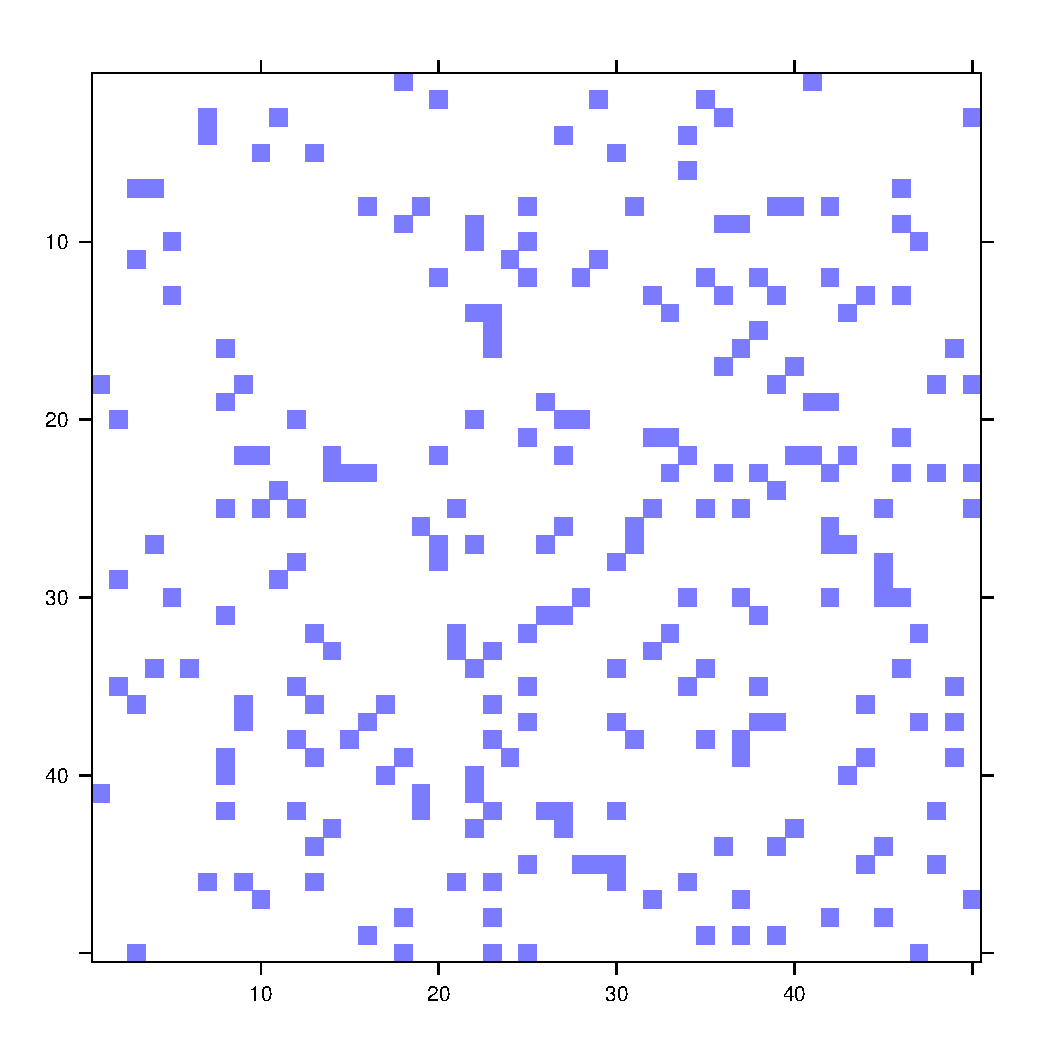
\includegraphics[width = .7in, height = .7in]{A3_beamer.pdf}};\pause
    
    
    %Draw ASE boxes
    \node[shape=rectangle, align = center, draw = black] (ASE1) at (.5, 2.5){\scriptsize{ASE}};
    \node[shape=rectangle, align = center, draw = black] (ASEg) at (.5, 0){\scriptsize{ASE}};
    \node[shape=rectangle, align = center, draw = black] (ASEm) at (.5, -2.5){\scriptsize{ASE}};
    
    %Draw ASE
    \node[shape=rectangle, align = center] (E1) at (3,2.5) {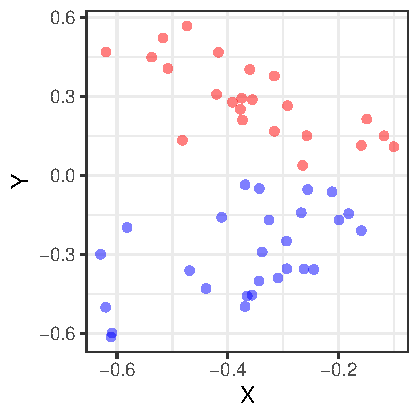
\includegraphics[width = .8in, height = .8in]{ase_0_three_vals.pdf}};
    \node[shape=rectangle, align = center] (Eg) at (3,0) {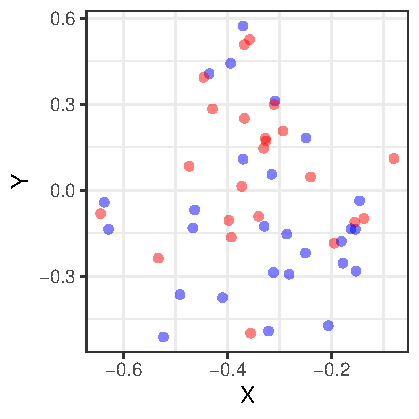
\includegraphics[width = 0.8in, height = .8in]{ase_5_three_vals.pdf}};
    \node[shape=rectangle, align = center] (Em) at (3,-2.5) {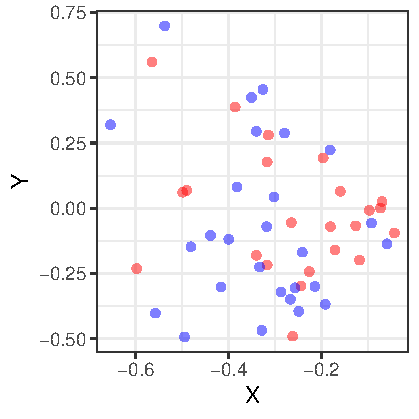
\includegraphics[width = 0.8in, height = .8in]{ase_1_three_vals.pdf}};
    
    %Draw arrows
    \draw (A1)--(ASE1); \draw[->] (ASE1)--(E1);
    \draw (Ag)--(ASEg); \draw[->] (ASEg)--(Eg);
    \draw (Am)--(ASEm); \draw[->] (ASEm)--(Em);
    \pause

    %draw bracket 
    \draw [decorate, decoration={brace,amplitude=10pt,raise=4pt}]
(4,3.5) -- (4,-3.5) node [black, midway, xshift=1.25cm, text width=1.5cm] {\footnotesize
Statistical Inference};
\end{tikzpicture}
\end{center}     
    
\end{frame}


\begin{frame}{Joint Spectral Embeddings}
\begin{center}
    \begin{tikzpicture}
    %Draw Networks
    \node[shape=rectangle, align = center] (G1) at (-4,2.5) {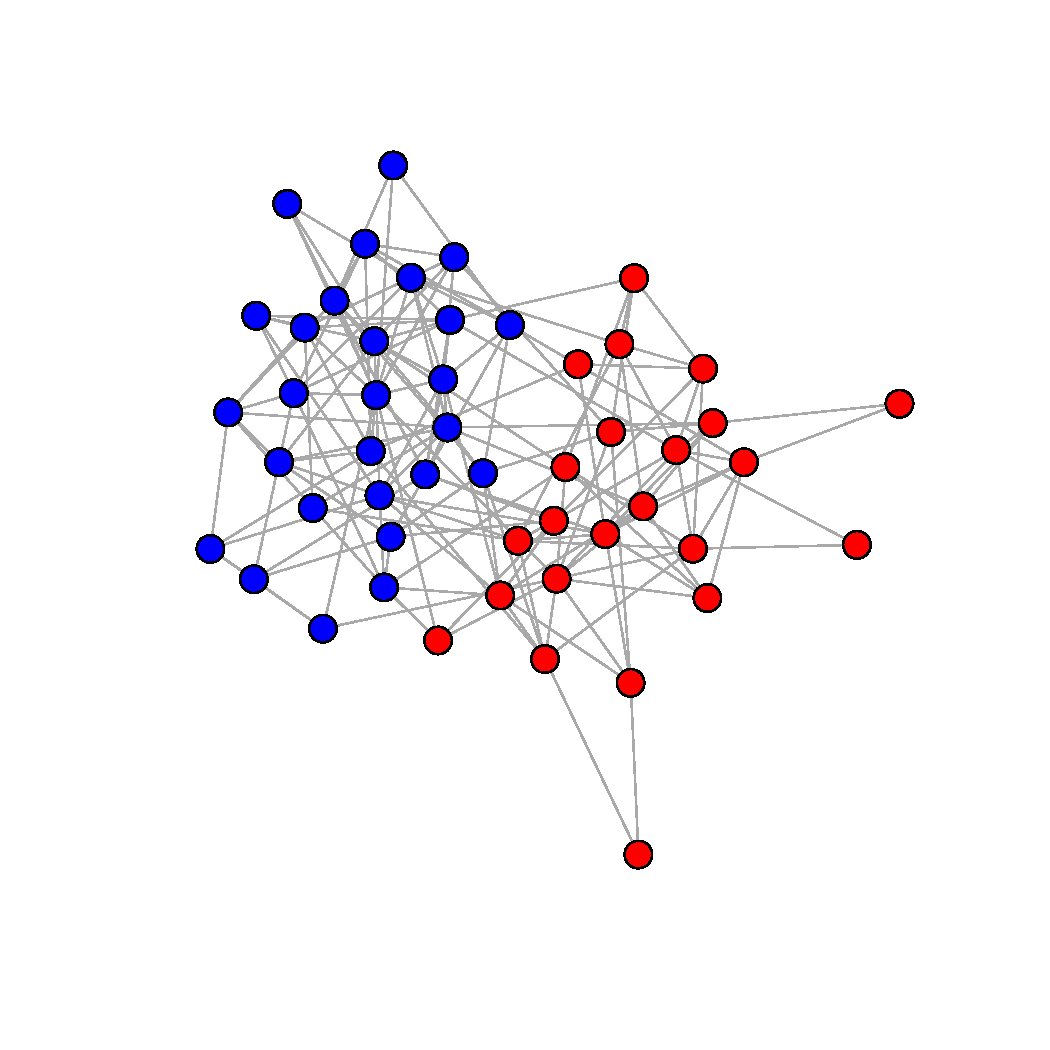
\includegraphics[width = 1in, height = 1in]{g1_beamer.pdf}};
    \node[shape=rectangle, align = center] (Gg) at (-4,0) {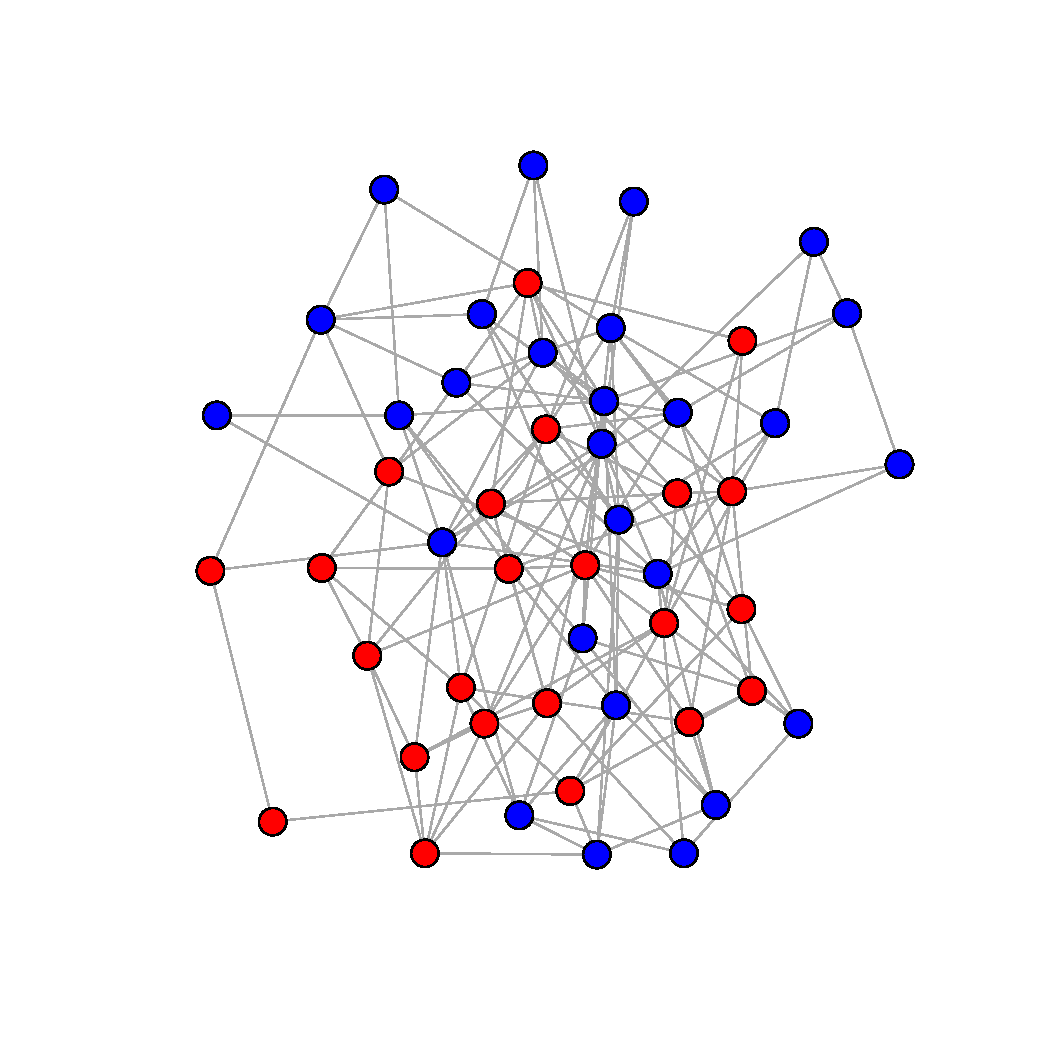
\includegraphics[width = 1in, height = 1in]{g2_beamer.pdf}};
    \node[shape=rectangle, align = center] (Gm) at (-4,-2.5) {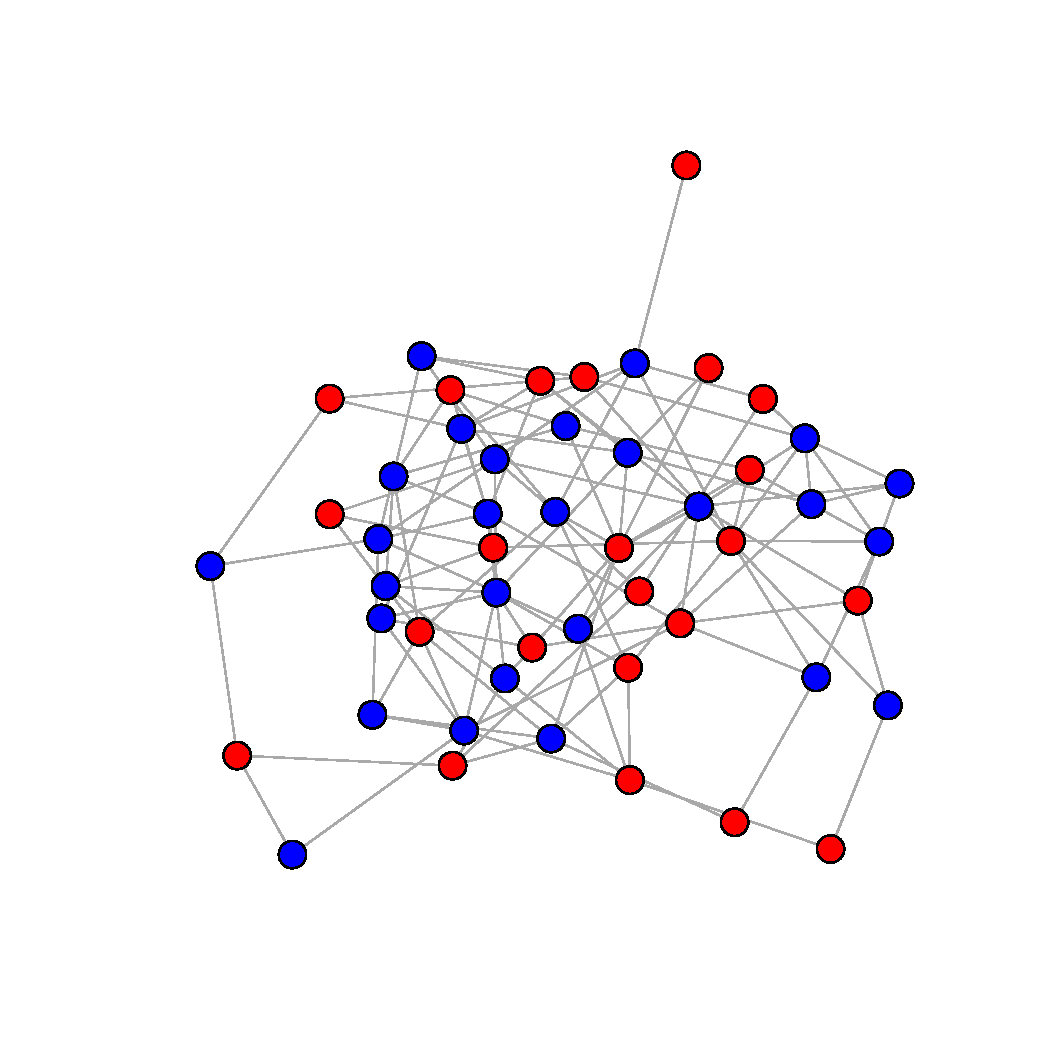
\includegraphics[width = 1in, height = 1in]{g3_beamer.pdf}};
    
    %Draw Adjacency Matrices
    \node[shape=rectangle, align = center] (A1) at (-2,2.5) {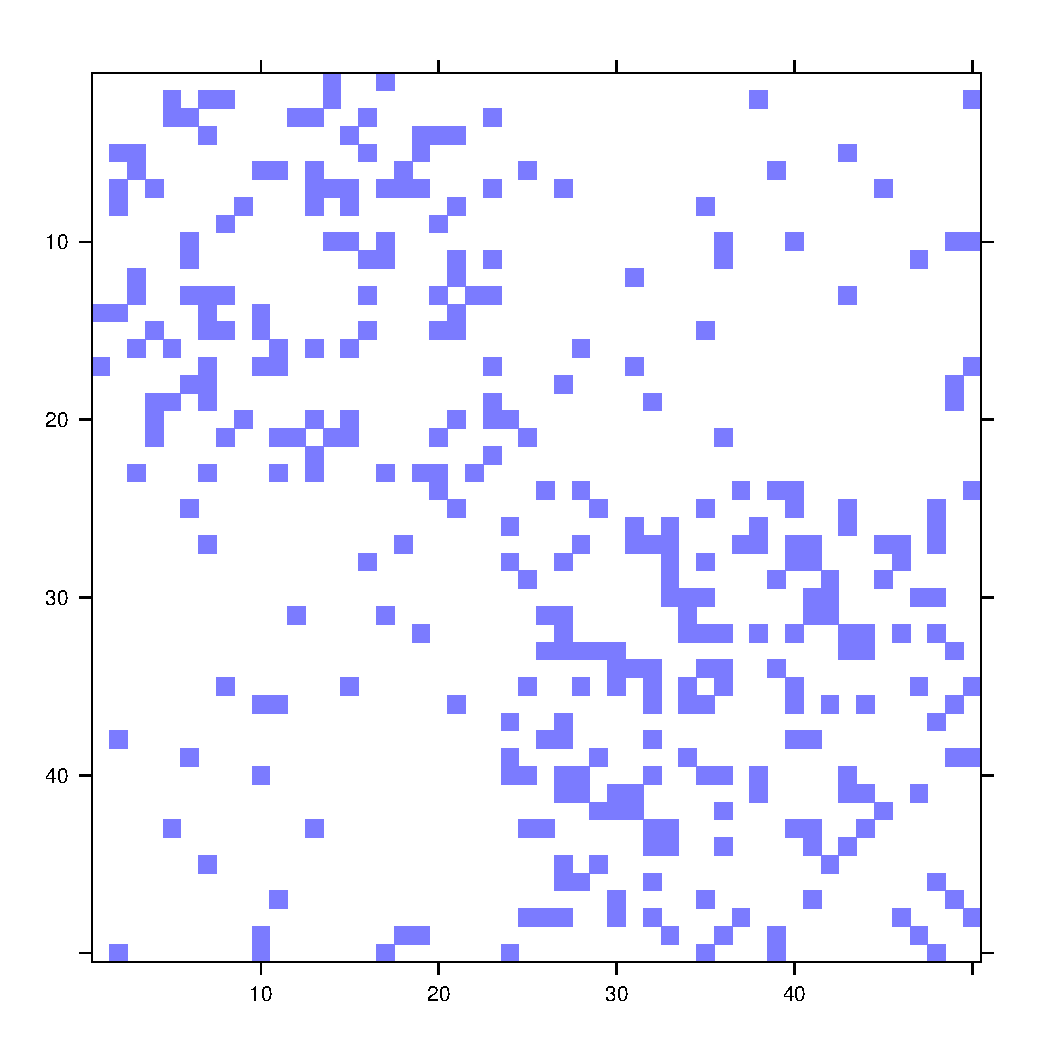
\includegraphics[width = .7in, height = .7in]{A1_beamer.pdf}};
    \node[shape=rectangle, align = center] (Ag) at (-2,0) {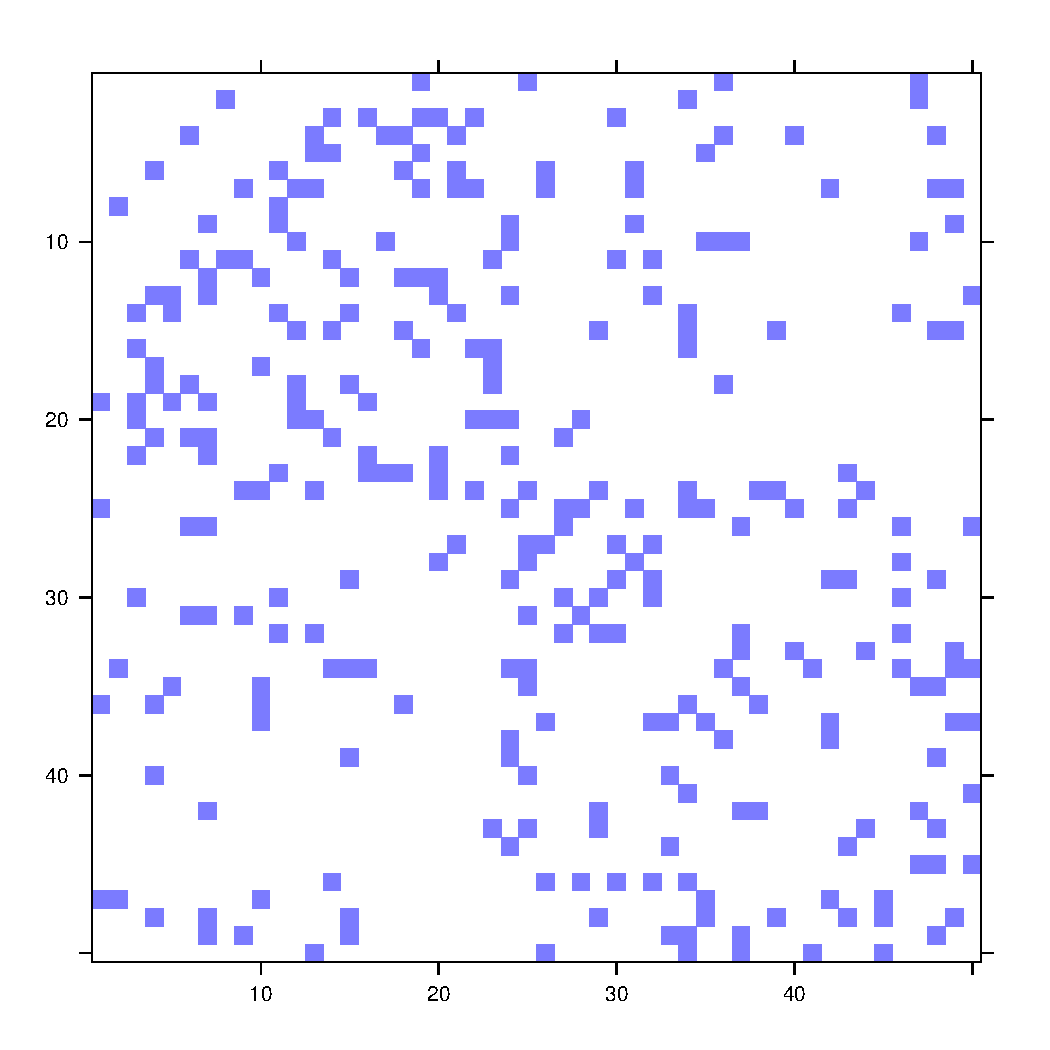
\includegraphics[width = .7in, height = .7in]{A2_beamer.pdf}};
    \node[shape=rectangle, align = center] (Am) at (-2,-2.5) {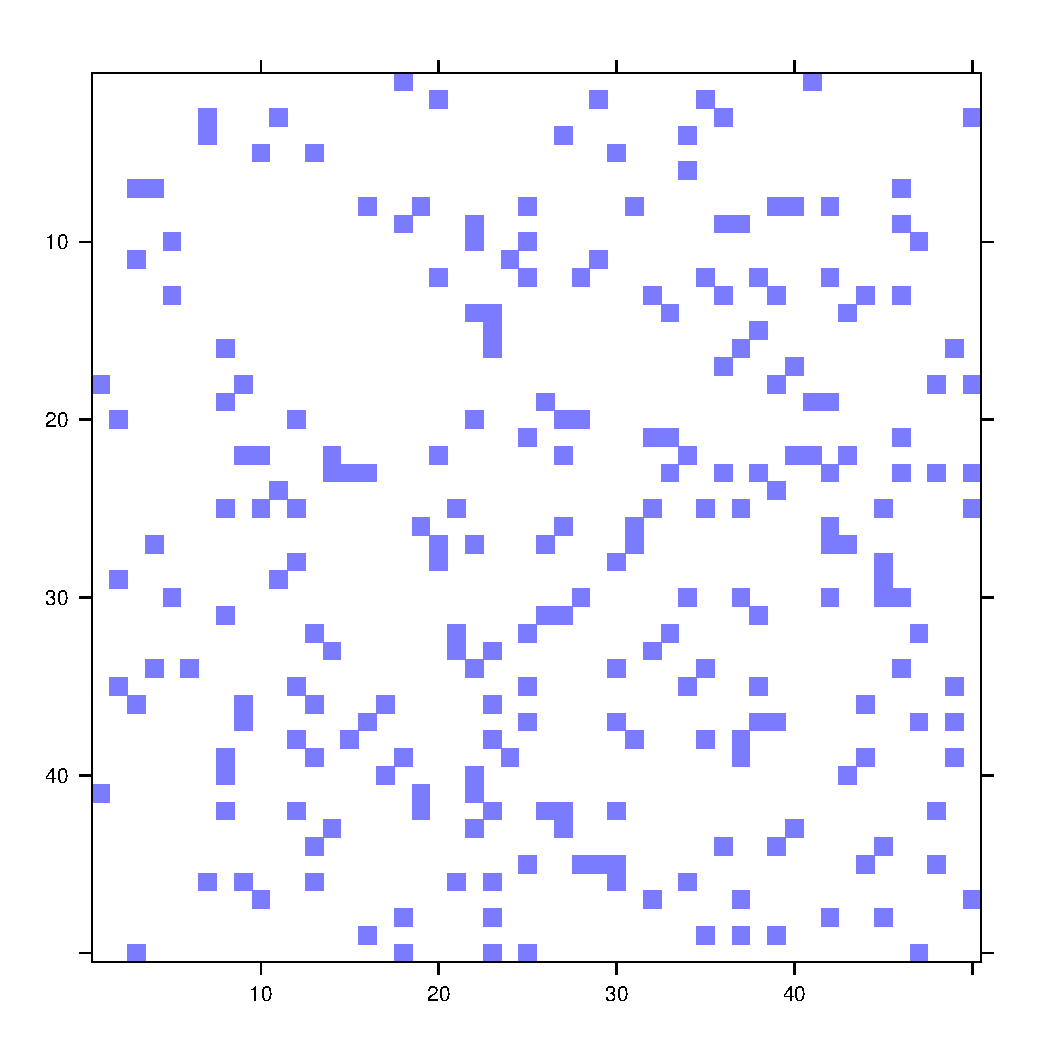
\includegraphics[width = .7in, height = .7in]{A3_beamer.pdf}};
    \pause
    
    %Draw Omni
    \node[shape=rectangle, align = center, draw = black, text width = 1.5cm] (Omni) at (0.5, 0){\scriptsize{Omnibus Embedding}};
    
    
    %Draw arrows
    %\draw (A1)--(-.4,.5); \draw[->] (1.4, 0.5)--(E1);
    %\draw (Ag)--(-.4, 0); \draw[->] (1.4, 0)--(Eg);
    %\draw (Am)--(-.4,-.5); \draw[->] (1.4, -0.5)--(Em);
    
    \draw (A1)--(-.4,0); \draw[->] (1.4, .2)--(E1);
    \draw (Ag)--(-.4, 0); \draw[->] (1.4, 0)--(Eg);
    \draw (Am)--(-.4,0); \draw[->] (1.4, -.2)--(Em);

    %Draw Omni
    \node[shape=rectangle, align = center] (E1) at (3,2.5) {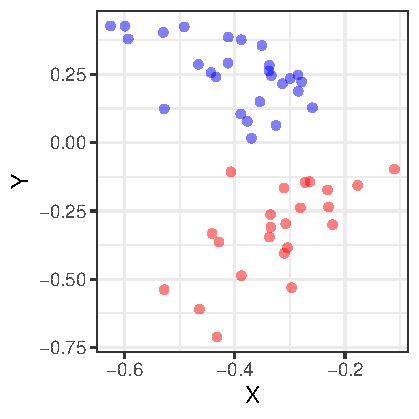
\includegraphics[width = .8in, height = .8in]{embedded_points_0_three_vals.pdf}};
    \node[shape=rectangle, align = center] (Eg) at (3,0) {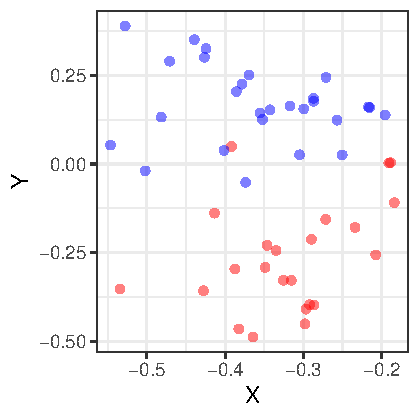
\includegraphics[width = 0.8in, height = .8in]{embedded_points_5_three_vals.pdf}};
    \node[shape=rectangle, align = center] (Em) at (3,-2.5) {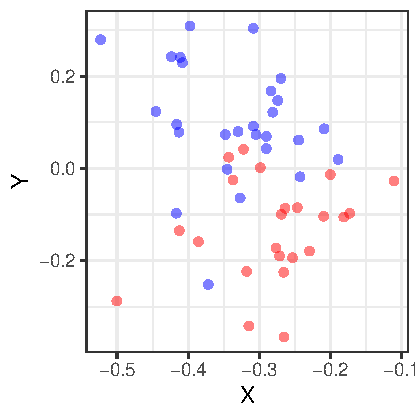
\includegraphics[width = 0.8in, height = .8in]{embedded_points_1_three_vals.pdf}};\pause
    
    
    %draw bracket 
    \draw [decorate, decoration={brace,amplitude=10pt,raise=4pt}]
(4,3.5) -- (4,-3.5) node [black,midway,xshift=1.25cm,text width=1.5cm] {\footnotesize{Statistical Inference}};\pause

    %Draw Omni
    \node[shape=rectangle, align = center, draw = yellow, line width = 1mm, text = black,  text width = 1.5cm] (Omni) at (0.5, 0){\scriptsize{Omnibus Embedding}};
    
\end{tikzpicture}
\end{center}     
\end{frame}


%--------------------------------------------------------------
\section{Bias-Variance Tradeoffs}

\begin{frame}{Analysis Framework}
    \begin{itemize}
        \item Consider $m$ graphs over a common vertex set $\mathcal{V}$ of size $n$ 
        \item Associate $v\in\mathcal{V}$ with a \textit{latent position} $\bvar{X}_v\in\mathbb{R}^d$
    \end{itemize}\pause
    \begin{block}{Inner Product Distribution}
    Let $F$ be a probability distribution over $\mathbb{R}^d$. We say $F$ is a \textit{$d$-dimensional inner product distribution} if all $\bvar{x},\bvar{y}\in \text{supp}(F)$ has the property $\bvar{x}^T\bvar{y}\in[0,1]$. 
    \end{block}
    \begin{itemize}
        \item Assume latent positions $\bvar{X}_1, \bvar{X}_2,\ldots, \bvar{X}_n\overset{i.i.d.}{\sim} F$. Organize in the rows of a matrix $\bvar{X} = [\bvar{X}_1\bvar{X}_2 \dots \bvar{X}_n]^T$. \pause
        \item Associate each network with a diagonal matrix $\bvar{C}^{(g)}\in\mathbb{R}_{\geq 0}^{d\times d}$ such that for all $\bvar{x}, \bvar{y}\in\text{supp}(F)$ and $g\in[m]$, $\bvar{x}^T\bvar{C}^{(g)}\bvar{y} \in [0,1]$. 
    \end{itemize}
    
\end{frame}


\begin{frame}{Eigen-Scaling Random Dot Product Graph}
    \begin{block}{Eigen-Scaling Random Dot Product Graph}
    \begin{itemize}
    \item Suppose that for $\bvar{y}\sim F$, $\Delta = \mathbb{E}[\bvar{yy}^T]$ is diagonal and full rank and the matrices $\{\bvar{C}^{(g)}\}_{g=1}^m$ satisfy $\min_{i\in[d]}\max_{g\in[m]}\bvar{C}^{(g)}_{ii} > 0$.\pause
    \item Then the random adjacency matrices $\{\bvar{A}^{(g)}\}_{g=1}^m $ are said to be jointly distributed according to the \textit{ESRDPG} with \textit{latent positions} $\bvar{X}$ iff $\{\bvar{A}_{ij}^{(g)}\}$ are conditionally independent with 
    \begin{align*}
        \mathbb{P}(\bvar{A}_{ij}^{(g)} = 1|\bvar{X}_i, \bvar{X}_j) = \bvar{X}_i^T\bvar{C}^{(g)}\bvar{X}_j
    \end{align*}
    \end{itemize}
    \end{block}\pause
    \begin{itemize}
        \item In essence, $\bvar{A}_{ij}^{(g)}|\bvar{X}\overset{ind.}{\sim} \text{Bern}(\bvar{X}_i^T\bvar{C}^{(g)}\bvar{X}_j)$. \pause
        \item Goal: Given $\{\bvar{A}^{(g)}\}_{g=1}^m$, estimate $\{\bvar{X}\sqrt{\bvar{C}^{(g)}}\}_{g=1}^m$
    \end{itemize}
\end{frame}


\begin{frame}{Individual Network Embedding Techniques}
\begin{itemize}
    \item First approach: ignore shared structure and individually embedd networks $\bvar{A}^{(g)}$ for $g\in[m]$.\pause
\end{itemize}
    \begin{block}{Adjacency Spectral Embedding (\cite{ASE})}
        Let $\bvar{A}^{(g)}$ have eigendecomposition 
        \begin{align*}
            \bvar{A}^{(g)} = [\bvar{U}_{\bvar{A}^{(g)}}|\tilde{\bvar{U}}_{\bvar{A}^{(g)}}][\bvar{S}_{\bvar{A}^{(g)}}\oplus \tilde{\bvar{S}}_{\bvar{A}^{(g)}}][\bvar{U}_{\bvar{A}^{(g)}}|\tilde{\bvar{U}}_{\bvar{A}^{(g)}}]^T
        \end{align*}
        where $\bvar{U}_{\bvar{A}^{(g)}}\in\mathbb{R}^{n\times d}$ and $\bvar{S}_{\bvar{A}^{(g)}}\in\mathbb{R}^{d\times d}$ contains the top $d$ eigenvalues of $\bvar{A}^{(g)}$. Then the ASE of $\bvar{A}^{(g)}$ is defined by $\text{ASE}(\bvar{A}^{(g)},d) = \bvar{U}_{\bvar{A}^{(g)}}\bvar{S}_{\bvar{A}^{(g)}}^{1/2}$.
        \end{block}
    \begin{itemize}
    \item Second approach: assume identical structure and embedd the sample mean matrix $\bar{\bvar{A}} =  m^{-1}\sum_{g=1}^m \bvar{A}^{(g)}$ by $\text{ASE}(\bar{\bvar{A}}, d)$. 
\end{itemize}
\end{frame}

\begin{frame}{Joint Network Embedding Techniques}
\begin{itemize}
        \item Thrid approach: \textit{jointly} embedd the networks $\{\bvar{A}^{(g)}\}_{g=1}^m$.
\end{itemize}
\begin{block}{Omnibus Embedding (\cite{OmniCLT})}
Let the \textit{omnibus matrix} be defined as
\begin{align*}
    \tilde{\bvar{A}} = \begin{bmatrix}
        \bvar{A}^{(1)} &\frac{1}{2}[\bvar{A}^{(1)} + \bvar{A}^{(2)}] & \dots & \frac{1}{2}[\bvar{A}^{(1)} + \bvar{A}^{(m)}]\\
        \frac{1}{2}[\bvar{A}^{(2)} + \bvar{A}^{(1)}] & \bvar{A}^{(2)} & \dots & \frac{1}{2}[\bvar{A}^{(2)} + \bvar{A}^{(m)}]\\
        \vdots & \vdots & \ddots & \vdots\\
        \frac{1}{2}[\bvar{A}^{(m)} + \bvar{A}^{(1)}] & \frac{1}{2}[\bvar{A}^{(m)} + \bvar{A}^{(2)}] & \dots & \bvar{A}^{(m)}
    \end{bmatrix}.
\end{align*}
Then the \textit{omnibus embedding} of $\{\bvar{A}^{(g)}\}_{g=1}^m$ is given by $\hat{\bvar{L}} = \text{ASE}(\tilde{\bvar{A}}, d)$. 
\end{block}
\begin{itemize}
        \item Notice $\hat{\bvar{L}}\in\mathbb{R}^{nm\times d}$ so each vertex has a latent position estimate for each graph.  
\end{itemize}
\end{frame}


\begin{frame}{Mean Squared Error Comparison}
    \begin{itemize}
        \item Suppose $\bvar{A}^{(1)}\sim\text{ER}(p)$ and $\bvar{A}^{(2)}\sim\text{ER}(c^2p)$
        \item Under ESRDPG: $\bvar{X} = \sqrt{p}\bvar{1}_n$,  $\bvar{C}^{(1)} = \bvar{I}$, and $\bvar{C}^{(2)} = c^2\bvar{I}$
    \end{itemize}\pause
\begin{center}
    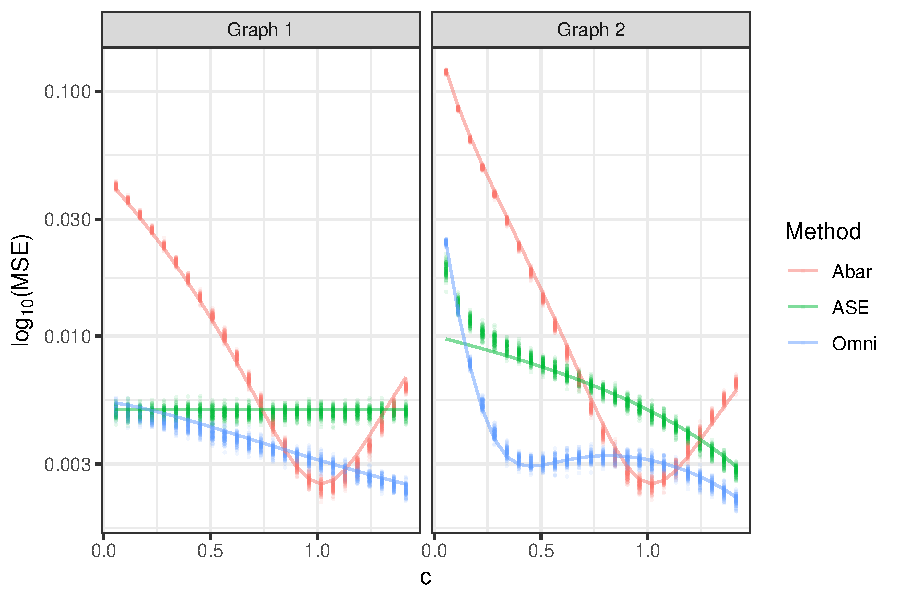
\includegraphics[width = 4in, height = 2.5in]{1d_mse.pdf}
\end{center}
\end{frame}


\begin{frame}{Main Results}
\begin{itemize}
    \item Let $\hat{\bvar{L}} = \text{ASE}(\tilde{\bvar{A}}, d)$ and $h = n(g-1) + i$ for $i\in[n]$ and $g\in[m]$ so that $\hat{\bvar{L}}_h \in\mathbb{R}^{d\times 1}$ is some row of $\hat{\bvar{L}}$ written as a column vector.\pause
\end{itemize}
    \begin{Theorem}
    \begin{itemize} 
        \item There exists diagonal matrices $\{\bvar{S}^{(g)}\}_{g=1}^m$ that only depend on $\{\bvar{C}^{(g)}\}_{g=1}^m$ and a sequence of orthogonal matrices $\{\tilde{\bvar{W}}_n\}_{n=1}^{\infty}$ such that 
        \begin{align}
            \hat{\bvar{L}}\tilde{\bvar{W}}_n - \bvar{L} &= (\bvar{S}^{(g)} - \sqrt{\bvar{C}^{(g)}})\bvar{X}_i + \bvar{R}_h
        \end{align}
        where $\bvar{R}_h$ is a residual.\pause 
        \item  $\bvar{R}_h$ satisfies $\max_{h\in[nm]}\|\bvar{R}_h\|_2 = O_{\mathbb{P}}\left(m^{3/2}\frac{\log nm}{\sqrt{n}}\right)$ and has asympoptic distribution
        \begin{align}
            \lim_{n\to\infty}\mathbb{P}\left[\sqrt{n}\bvar{R}_h\leq \bvar{x}\right] = \int_{\text{supp}(F)}\Phi(\bvar{x}; \bvar{0}, \Sigma_g(\bvar{y}))dF(\bvar{y}). 
        \end{align}
    \end{itemize}
    \end{Theorem}
\end{frame}

%--------------------------------------------------------------
\section{Statistical Ramifications}

\begin{frame}{Simulation Experiment}

    \begin{block}{Simulation Design}
        \begin{enumerate}
            \item Draw $\bvar{X}_1, \ldots \bvar{X}_n \overset{i.i.d}{\sim} F$ where $F$ corresponds to a two-group SBM with paramters $(a = 0.25, b = 0.05)$. 
            \item For $t\in[0,1]$, draw $(\{\bvar{A}^{(g)}\}_{g=1}^2, \bvar{X})\sim \text{ESRDPG}(F, n, \{\bvar{C}^{(g)}\}_{g=1}^m)$ with 
               \begin{align*}
                    \bvar{C}^{(1)} = \bvar{I} \quad \quad \bvar{C}^{(2)} := \bvar{C}(t) = \begin{bmatrix} 1 + t & 0\\ 0 & 1 - t \end{bmatrix}
                \end{align*}
            \item Jointly embedd $\hat{\bvar{L}} = \text{ASE}(\tilde{\bvar{A}}, d)$
        \end{enumerate}
    \end{block}
 \begin{itemize}
    \item At $t = 0$, $\bvar{A}^{(2)}$ is a SBM and at $t = 1$, $\bvar{A}^{(2)}$ is an Erd\"{o}s-R\'{e}yni graph with paramter $p = 0.3$.\pause
    \item Goal: Analyze techniques that utilize $\hat{\bvar{L}}$ for statistical inference. 
 \end{itemize}   
\end{frame}

\begin{frame}{Community Detection}
    \begin{center}
        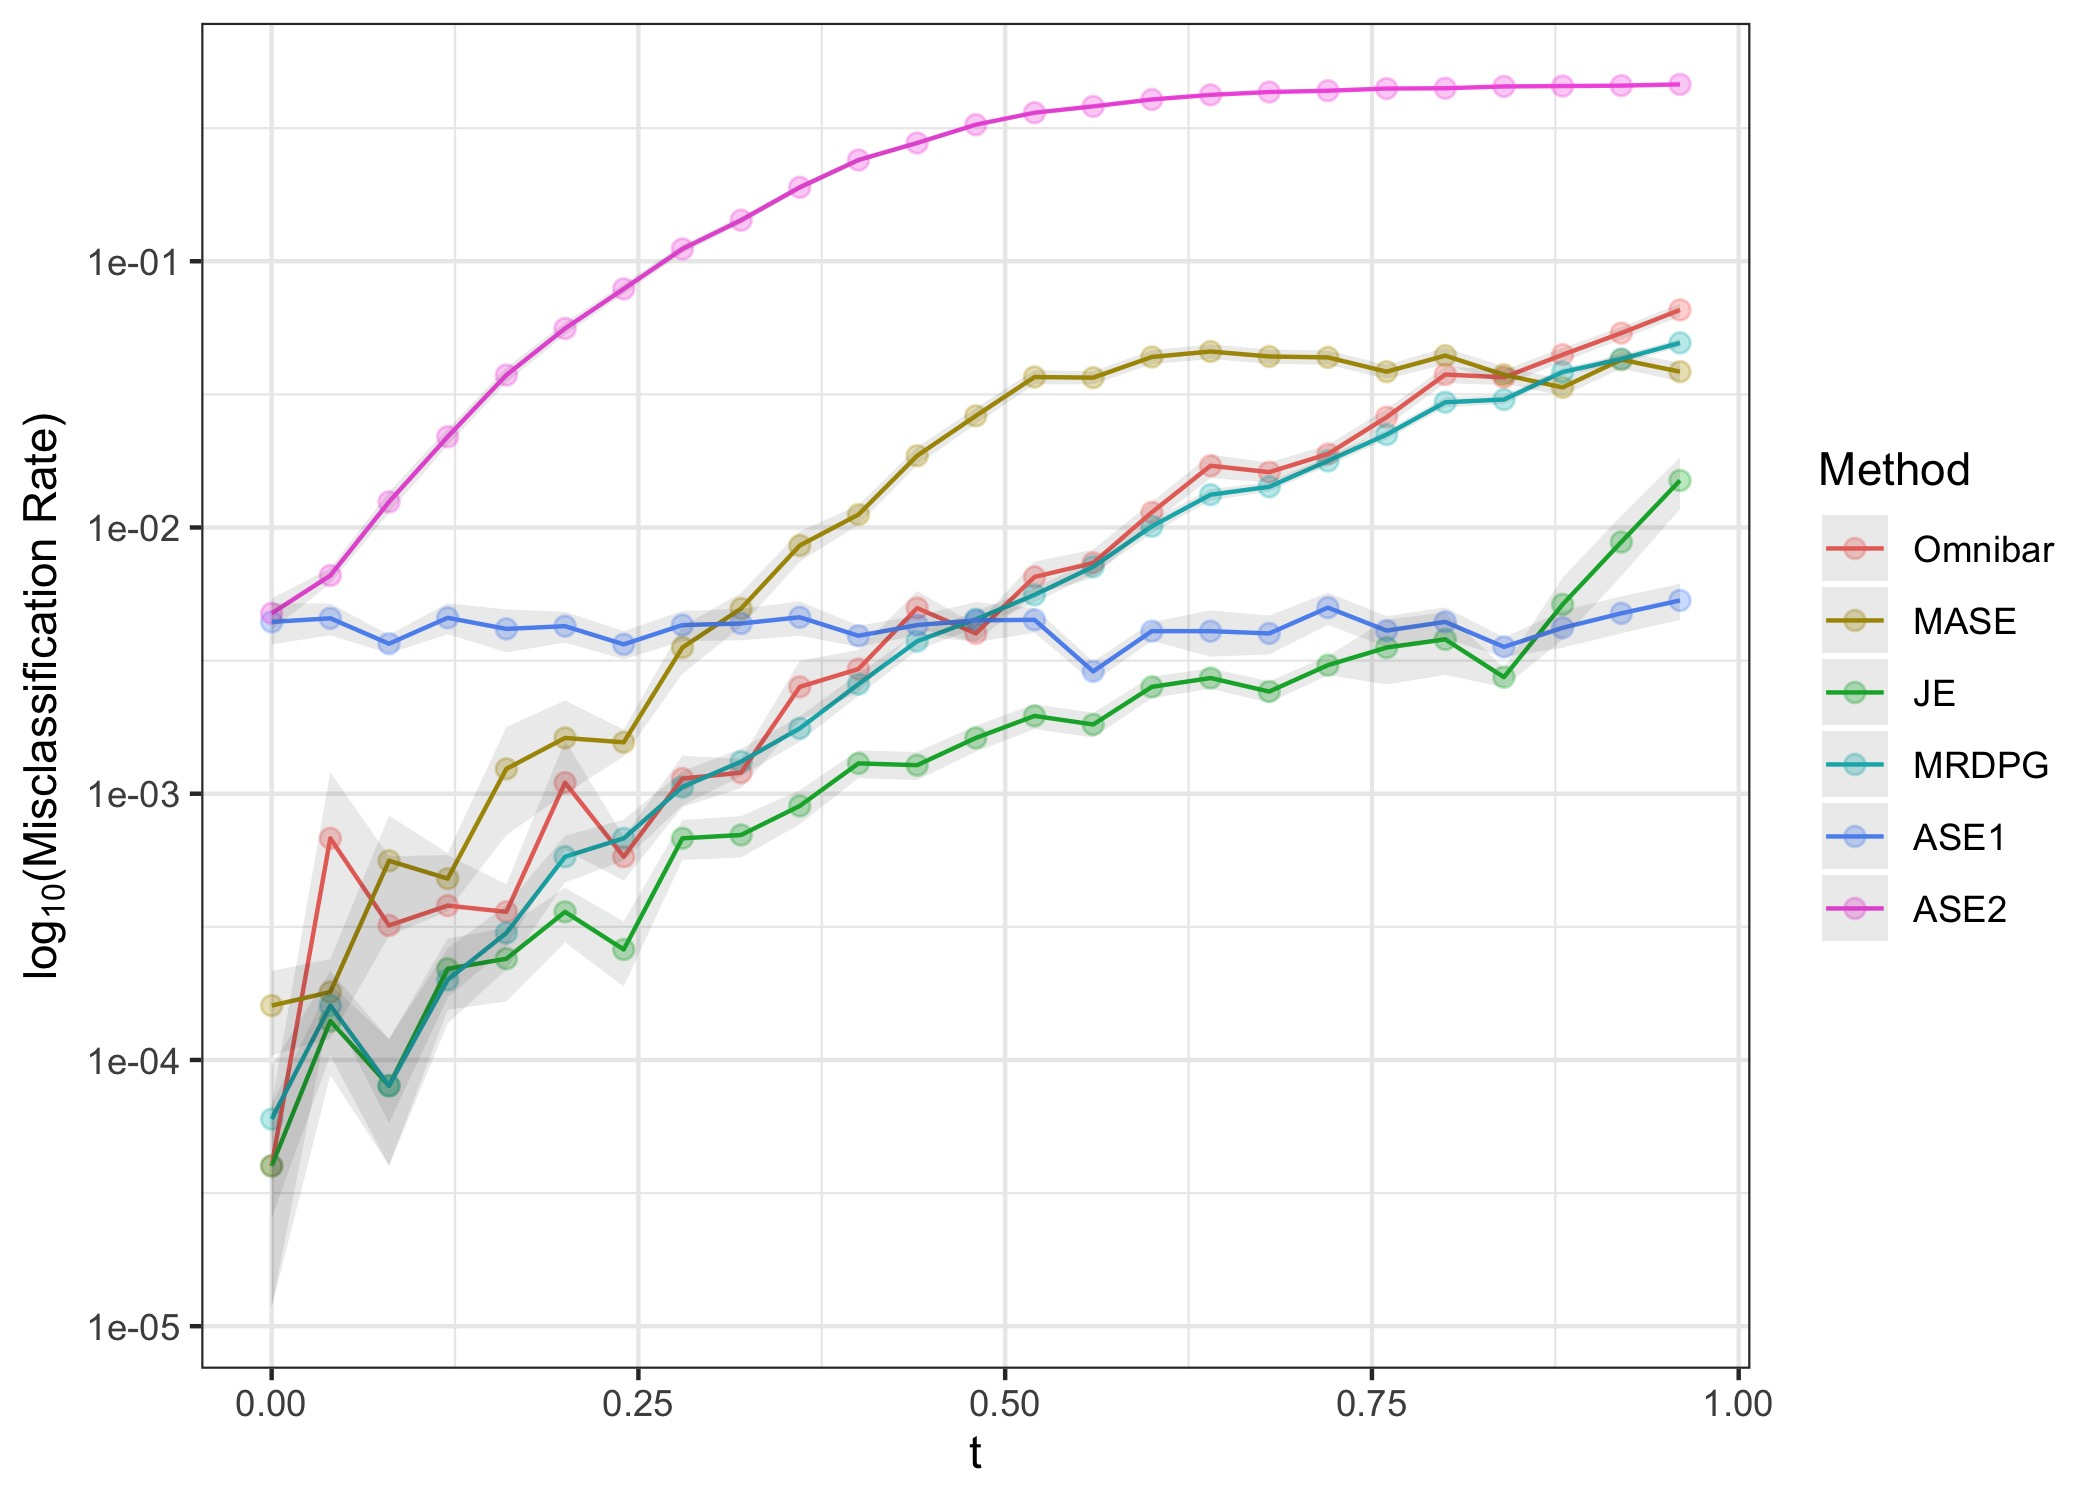
\includegraphics[width = 3in, height = 2in]{multiple_methods_mc_comp.jpeg}
    \end{center}
\end{frame}

\begin{frame}{Two Graph Hypothesis Testing}
    \begin{center}
        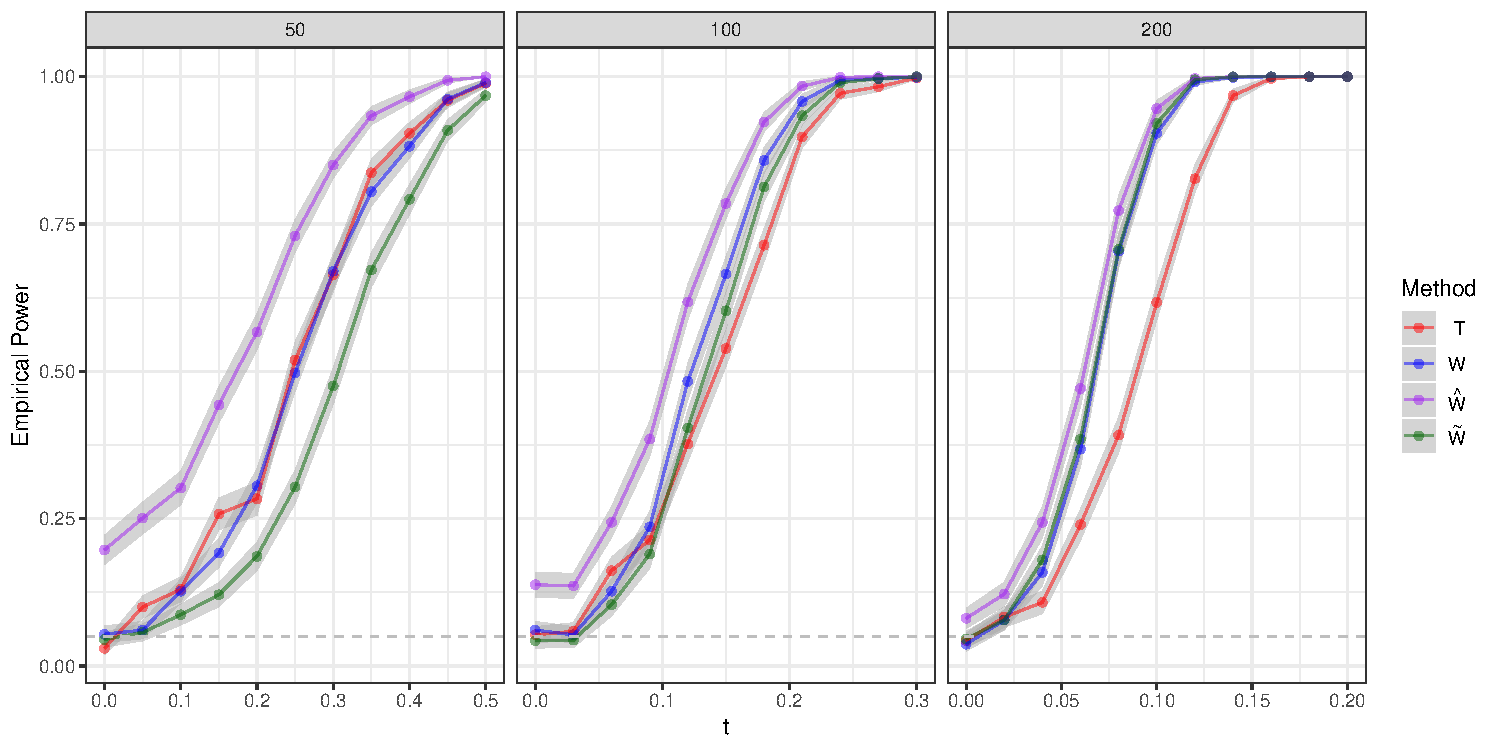
\includegraphics[width = 3in, height = 2in]{empirical_power_oracle_correction_variable_t.pdf}
    \end{center}
\end{frame}


%--------------------------------------------------------------
\section{Conclusion}

\begin{frame}{Conclusion \& Future Work}
    \begin{itemize}
        \item Preprint available: \url{https://arxiv.org/abs/2005.02511}
    \end{itemize}
\end{frame}


\nocite{*}
\begin{frame}[t,allowframebreaks]
  \frametitle{References}
  \printbibliography
 \end{frame}
%--------------------------------------------------------------







\end{document}


